% ============================================================================
% KnotTransformer — Length-Generalizing Neural Parameterization
%                    for B-Spline Curve Interpolation
% ============================================================================
% Ready for Overleaf upload. Compile with pdflatex.
% For submission: adjust \documentclass to match target venue.
% ============================================================================

\documentclass[11pt, a4paper]{article}

% ── Packages ────────────────────────────────────────────────────────────────
\usepackage[utf8]{inputenc}
\usepackage[T1]{fontenc}
\usepackage{amsmath, amssymb, amsthm}
\usepackage{mathtools}
\usepackage{bm}
\usepackage{booktabs}
\usepackage{multirow}
\usepackage{graphicx}
\usepackage{xcolor}
\usepackage{tikz}
\usepackage{pgfplots}
\usepackage{algorithm}
\usepackage{algpseudocode}
\usepackage{hyperref}
\usepackage[margin=1in]{geometry}
\usepackage{caption}
\usepackage{subcaption}

% TikZ libraries
\usetikzlibrary{arrows.meta, positioning, calc, decorations.pathreplacing,
                 fit, backgrounds, shapes.geometric, matrix}
\pgfplotsset{compat=1.18}

% ── Custom colors ───────────────────────────────────────────────────────────
\definecolor{cPurple}{HTML}{7F77DD}
\definecolor{cRed}{HTML}{E24B4A}
\definecolor{cGreen}{HTML}{1D9E75}
\definecolor{cAmber}{HTML}{EF9F27}
\definecolor{cBlue}{HTML}{2E86DE}
\definecolor{cGray}{HTML}{888888}

% ── Theorem environments ────────────────────────────────────────────────────
\newtheorem{definition}{Definition}
\newtheorem{proposition}{Proposition}
\newtheorem{remark}{Remark}

% ── Shortcuts ───────────────────────────────────────────────────────────────
\newcommand{\R}{\mathbb{R}}
\newcommand{\bC}{\mathbf{C}}
\newcommand{\bD}{\mathbf{D}}
\newcommand{\bP}{\mathbf{P}}
\newcommand{\bA}{\mathbf{A}}
\newcommand{\bu}{\mathbf{u}}
\newcommand{\bk}{\mathbf{k}}
\newcommand{\bQ}{\mathbf{Q}}
\newcommand{\norm}[1]{\lVert #1 \rVert}
\DeclareMathOperator{\softplus}{softplus}
\DeclareMathOperator{\cumsum}{cumsum}
\DeclareMathOperator{\attn}{Attn}

% ════════════════════════════════════════════════════════════════════════════
\title{%
  \textbf{Length-Generalizing Neural Parameterization\\
  for B-Spline Curve Interpolation}\\[6pt]
  \large A Transformer Approach to Self-Supervised Knot Placement
}
\author{%
  [Author Name]\\
  \textit{[Institution]}\\
  \texttt{[email]}
  \and
  Vinai Chhetri\\
  \textit{[Institution]}\\
  \texttt{[email]}
}
\date{}

% ════════════════════════════════════════════════════════════════════════════
\begin{document}
\maketitle

% ── Abstract ────────────────────────────────────────────────────────────────
\begin{abstract}
Selecting the knot vector for B-spline interpolation directly determines the
smoothness of the resulting curve. Prior work trained per-length neural
networks to predict interior knots that minimize total curvature, but
required a separate model for each point-sequence length. We replace these
fixed-size MLPs with a single encoder--decoder Transformer that accepts
variable-length point sequences via padding masks and outputs variable-length
knot vectors via learned queries. Trained on sequences of length $N \in
\{4,5\}$ using a two-phase self-supervised pipeline (chordal pretraining
followed by direct curvature minimization), the model generalizes to
held-out lengths $N = 6, 7, 8$ without retraining. On 500-sample test sets,
the model achieves a 75.7\% $\pm$ 4.0\% win rate against the chordal
heuristic at $N = 6$ (median curvature ratio 0.295), comparable to per-length
specialist models trained explicitly for that length. On hard test cases
(chordal $\kappa > 1000$), the model wins 90.4\% $\pm$ 1.6\% of the time
with curvature 2--6\% of the baseline. Performance degrades gracefully to
$N = 8$, three steps beyond the training distribution, demonstrating
length-invariant geometric reasoning rather than per-length memorization.
\end{abstract}

\vspace{4pt}
\noindent\textbf{Keywords:}
B-spline interpolation, knot placement, self-supervised learning,
transformer, curvature minimization, length generalization.


% ════════════════════════════════════════════════════════════════════════════
\section{Introduction}
\label{sec:intro}

A fundamental task in computer-aided geometric design (CAGD) is the
construction of a smooth curve that interpolates a given set of ordered
points. The standard tool is the clamped cubic B-spline, whose shape is
governed by a \emph{knot vector}---a non-decreasing sequence of real numbers
that parameterizes how the curve flows through its data points. For $N$ data
points, the spline has $K = N - 2$ interior knots, and these $K$ numbers are
the only free design variables: once the knots are chosen, the control
points and thus the entire curve are uniquely determined by a linear
solve~\cite{deBoor1978}.

Classical heuristics---uniform, chordal, and centripetal
parameterization~\cite{Lee1989}---assign knots based on inter-point
distances. These are fast and reasonable, but they do not optimize any
fairness criterion. The gap between heuristic and optimal knot placement was
studied by~\cite{Chhetri2024}, who trained neural networks to predict
curvature-minimizing knots via a self-supervised energy objective. Their
approach demonstrated that a network can learn to produce knot vectors whose
resulting curves have significantly lower total curvature than the chordal
baseline. However, their architecture required a \emph{separate} network for
each value of $K$ (and thus each sequence length $N$), a limitation they
explicitly identified as future work~\cite[§7.3]{Chhetri2024}:

\begin{quote}
\emph{``We were only able to create neural networks that could handle
fixed-size inputs. It cannot interpolate minimal-energy B-splines on
an arbitrary number of points.''}
\end{quote}

We address this limitation by replacing the per-length MLPs with a single
encoder--decoder Transformer of the DETR family~\cite{Carion2020}. Our
model accepts any $N \leq 10$ via padding masks, outputs up to $K = 6$
interior knots via learned queries, and is trained end-to-end using the same
two-phase pipeline. The central finding: \textbf{a model trained on
$N \in \{4,5\}$ generalizes to held-out lengths $N = 6, 7, 8$}, matching
per-length specialists at $N = 6$ and degrading gracefully beyond.

\begin{figure}[t]
\centering
% ── Pipeline overview (TikZ) ──────────────────────────────────────────
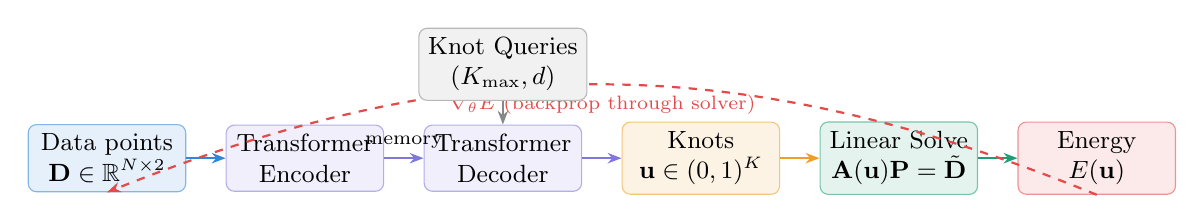
\begin{tikzpicture}[
    node distance=0.5cm,
    box/.style={draw, rounded corners=3pt, minimum height=0.7cm,
                minimum width=2.0cm, font=\small, align=center,
                fill=#1!12, draw=#1!60},
    arr/.style={-{Stealth[length=5pt]}, thick, draw=#1},
    every node/.style={font=\small},
  ]
  % Forward pass
  \node[box=cBlue]                 (pts)  {Data points\\$\bD \in \R^{N \times 2}$};
  \node[box=cPurple, right=of pts] (enc)  {Transformer\\Encoder};
  \node[box=cPurple, right=of enc] (dec)  {Transformer\\Decoder};
  \node[box=cAmber,  right=of dec] (kn)   {Knots\\$\bu \in (0,1)^K$};
  \node[box=cGreen,  right=of kn]  (sol)  {Linear Solve\\$\bA(\bu)\bP = \tilde\bD$};
  \node[box=cRed,    right=of sol] (eng)  {Energy\\$E(\bu)$};

  \draw[arr=cBlue]   (pts) -- (enc);
  \draw[arr=cPurple] (enc) -- (dec) node[midway, above, font=\scriptsize]
                     {memory};
  \draw[arr=cPurple] (dec) -- (kn);
  \draw[arr=cAmber]  (kn)  -- (sol);
  \draw[arr=cGreen]  (sol) -- (eng);

  % Backward pass (gradient)
  \draw[arr=cRed, dashed, bend right=22]
    (eng.south) to node[below, font=\scriptsize, text=cRed]
    {$\nabla_\theta E$ (backprop through solver)} (pts.south);

  % Queries
  \node[box=cGray, above=0.3cm of dec, minimum width=1.6cm]
    (q) {Knot Queries\\$(K_{\max}, d)$};
  \draw[arr=cGray] (q) -- (dec);
\end{tikzpicture}
\caption{%
  The full forward pass. Data points enter the encoder; learned knot
  queries cross-attend to the encoded geometry in the decoder; the output
  head produces ordered knots; the differentiable solver builds the
  curve and computes its energy. Gradients flow backward through
  the entire chain (dashed), including implicit differentiation through
  the linear solve.%
}
\label{fig:pipeline}
\end{figure}


% ════════════════════════════════════════════════════════════════════════════
\section{Mathematical Background}
\label{sec:background}

% ── 2.1 B-spline curves ────────────────────────────────────────────────────
\subsection{B-Spline Curves}

\begin{definition}[Clamped Cubic B-Spline]
Given a non-decreasing \emph{knot vector}
$U = \{\underbrace{0,\dots,0}_{4},\; u_1,\dots,u_K,\;
       \underbrace{1,\dots,1}_{4}\}$
with $K$ interior knots in $(0,1)$ and $n+1 = K + 4$ control points
$\bP_0,\dots,\bP_n \in \R^d$, the \emph{clamped cubic B-spline curve} is
\begin{equation}
  \bC(t) = \sum_{i=0}^{n} N_{i,3}(t)\;\bP_i, \qquad t \in [0,1],
  \label{eq:bspline}
\end{equation}
where $N_{i,p}$ are the Cox--de~Boor basis functions of degree~$p$.
\end{definition}

The basis functions are defined recursively. The zeroth-degree functions are
indicator functions on knot spans:
\begin{equation}
  N_{i,0}(t) =
  \begin{cases}
    1 & \text{if } u_i \leq t < u_{i+1},\\
    0 & \text{otherwise},
  \end{cases}
  \label{eq:basis0}
\end{equation}
and for $p \geq 1$:
\begin{equation}
  N_{i,p}(t) =
  \frac{t - u_i}{u_{i+p} - u_i}\,N_{i,p-1}(t)
  + \frac{u_{i+p+1} - t}{u_{i+p+1} - u_{i+1}}\,N_{i+1,p-1}(t),
  \label{eq:coxdeboor}
\end{equation}
with the convention $0/0 \equiv 0$. The key structural properties are:

\begin{itemize}
  \item \textbf{Non-negativity and partition of unity:}
        $N_{i,p}(t) \geq 0$ and $\sum_i N_{i,p}(t) = 1$.
  \item \textbf{Local support:}
        $N_{i,p}(t) = 0$ for $t \notin [u_i, u_{i+p+1})$.
  \item \textbf{Clamping:}
        The multiplicity-4 end knots force
        $\bC(0) = \bP_0$ and $\bC(1) = \bP_n$.
\end{itemize}

For $N$ data points the dimension count is:
\begin{equation}
  \underbrace{|U| = N + 6}_{\text{knot vector}},\qquad
  \underbrace{n + 1 = N + 2}_{\text{control points}},\qquad
  \underbrace{K = N - 2}_{\text{interior knots (free dials)}}.
  \label{eq:dimensions}
\end{equation}


% ── 2.2 Interpolation as a linear solve ────────────────────────────────────
\subsection{Interpolation as a Linear Solve}
\label{sec:interp}

Given $N$ ordered data points $\bD_0, \dots, \bD_{N-1} \in \R^2$ and
parameter values $\bar{t}_k$ (determined by the knots), the interpolation
conditions are:
\begin{equation}
  \bC(\bar{t}_k) = \sum_{i=0}^{N+1} N_{i,3}(\bar{t}_k)\,\bP_i = \bD_k,
  \qquad k = 0,\dots,N-1.
  \label{eq:interp_cond}
\end{equation}
Together with natural end conditions
$\bC''(0) = \bC''(1) = \mathbf{0}$, this yields a square
$(N{+}2) \times (N{+}2)$ linear system:
\begin{equation}
  \boxed{\;\bA(\bu)\,\bP = \tilde{\bD}\;}
  \label{eq:linsys}
\end{equation}
where $\bA(\bu)$ is the collocation matrix (built from basis-function
evaluations at the data parameters), $\bP$ is the $(N{+}2) \times 2$
control-point matrix, and $\tilde{\bD}$ stacks the data points with two
zero rows for the end conditions.

\begin{remark}[Fit is Free]
\label{rem:fit_free}
For \emph{any} valid knot vector $\bu$, the linear system~\eqref{eq:linsys}
has a unique solution $\bP(\bu) = \bA(\bu)^{-1}\tilde{\bD}$. Every
resulting curve passes exactly through all data points. There is no
fit-vs-smoothness trade-off: we are choosing among a family of perfectly
interpolating curves, seeking the smoothest.
\end{remark}


% ── 2.3 Derivatives and curvature ──────────────────────────────────────────
\subsection{Derivatives and Curvature}

The derivative of a degree-$p$ B-spline is a degree-$(p{-}1)$ B-spline
with \emph{first-difference} control points:
\begin{equation}
  \bC'(t) = \sum_i N_{i,p-1}(t)\,\bQ_i,\qquad
  \bQ_i = \frac{p}{u_{i+p+1} - u_{i+1}}(\bP_{i+1} - \bP_i).
  \label{eq:deriv1}
\end{equation}
The second derivative follows by repeating:
\begin{equation}
  \bC''(t) = \sum_i N_{i,p-2}(t)\,\bR_i,\qquad
  \bR_i = \frac{p{-}1}{u_{i+p} - u_{i+1}}(\bQ_{i+1} - \bQ_i).
  \label{eq:deriv2}
\end{equation}

\textbf{The mechanism linking knots to curvature.}
The knot differences $u_{i+p+1} - u_{i+1}$ appear in the
\emph{denominator} of~\eqref{eq:deriv1}. Moving two knots close together
increases the magnitude of the corresponding $\bQ_i$, accelerating the
curve through that region and potentially increasing curvature. The
optimization seeks the knot spacing that balances these derivative
magnitudes globally.

For a parametric planar curve $\bC(t) = (x(t), y(t))$, the signed
curvature is:
\begin{equation}
  \kappa(t) = \frac{x'y'' - y'x''}{\bigl(x'^2 + y'^2\bigr)^{3/2}},
  \label{eq:curvature}
\end{equation}
and the total bending energy is the integral of squared curvature weighted
by arc-length element:
\begin{equation}
  E_{\text{curv}}(\bu) =
    \int_0^1 \kappa(t)^2\,\norm{\bC'(t)}\,dt
  \approx \frac{1}{M}\sum_{j=1}^{M}
    \kappa(t_j)^2\,\norm{\bC'(t_j)},
  \label{eq:energy}
\end{equation}
approximated by Newton--Cotes quadrature with $M = 100$ samples.

\begin{remark}[Numerical Instability]
When $\norm{\bC'(t)} \to 0$ (near a cusp), $\kappa$ diverges via the
$({\cdot})^{3/2}$ denominator. This produces rare but extreme energy
values (up to $10^8$ in our data), necessitating energy capping and
dataset filtering during training (Section~\ref{sec:training}).
\end{remark}


% ── 2.4 The optimization problem ───────────────────────────────────────────
\subsection{The Optimization Landscape}

Composing the chain, the energy is a scalar function of the interior knots:
\begin{equation}
  \bu \;\xrightarrow{\;\bA^{-1}\;}
  \bP(\bu) \;\xrightarrow{\;\text{derivs + quadrature}\;}
  E(\bu) \in \R.
  \label{eq:chain}
\end{equation}
This landscape is non-convex---multiple local minima exist, and the
$({\cdot})^{3/2}$ nonlinearity creates ridges near degenerate
configurations. Heuristics like chordal parameterization provide a single
point on this landscape; optimization methods (gradient descent,
line search) walk downhill from a starting point to a local minimum; our
neural model learns to jump directly near a good minimum in one forward
pass.


% ════════════════════════════════════════════════════════════════════════════
\section{Classical Baselines}
\label{sec:baselines}

The chordal heuristic~\cite{Lee1989} sets the $k$-th parameter
proportional to cumulative chord lengths:
\begin{equation}
  \bar{t}_k = \frac{\sum_{j=1}^{k} \norm{\bD_j - \bD_{j-1}}}
                    {\sum_{j=1}^{N-1} \norm{\bD_j - \bD_{j-1}}},
  \qquad k = 1, \dots, N-2.
  \label{eq:chordal}
\end{equation}
This accounts for inter-point distances but ignores turning angles and
curvature. The centripetal variant replaces chord lengths with their
square roots, damping the influence of large gaps.


% ════════════════════════════════════════════════════════════════════════════
\section{The KnotTransformer Architecture}
\label{sec:arch}

\begin{figure}[t]
\centering
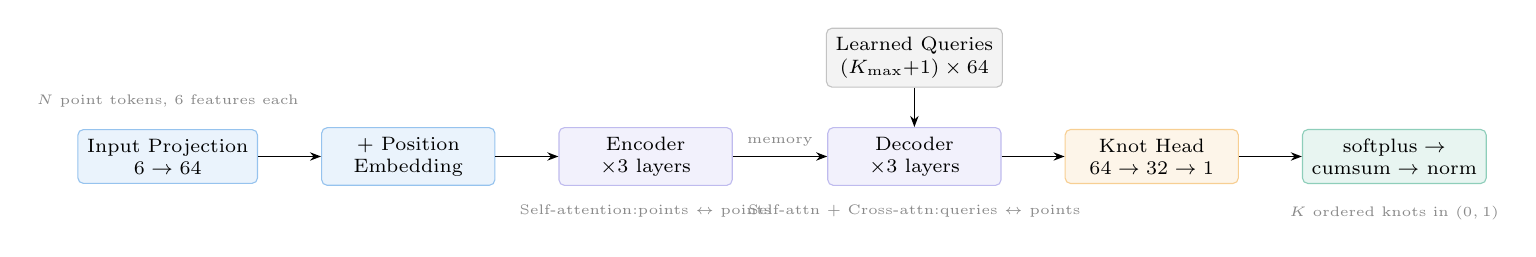
\begin{tikzpicture}[
    node distance=0.4cm and 0.6cm,
    block/.style={draw, rounded corners=2pt, minimum width=2.2cm,
                  minimum height=0.55cm, font=\scriptsize, align=center,
                  fill=#1!10, draw=#1!50},
    arr/.style={-{Stealth[length=4pt]}, semithick},
    lbl/.style={font=\tiny, text=cGray},
  ]
  % ── INPUT ──
  \node[block=cBlue] (inp) {Input Projection\\$6 \to 64$};
  \node[lbl, above=0.15cm of inp] {$N$ point tokens, 6 features each};

  % ── POS EMBED ──
  \node[block=cBlue, right=0.8cm of inp] (pos) {$+$ Position\\Embedding};
  \draw[arr] (inp) -- (pos);

  % ── ENCODER ──
  \node[block=cPurple, right=0.8cm of pos] (enc) {Encoder\\$\times 3$ layers};
  \draw[arr] (pos) -- (enc);

  % ── DECODER ──
  \node[block=cPurple, right=1.2cm of enc] (dec) {Decoder\\$\times 3$ layers};
  \draw[arr] (enc) -- (dec) node[midway, above, lbl] {memory};

  % ── QUERIES ──
  \node[block=cGray, above=0.5cm of dec] (q) {Learned Queries\\$(K_{\max}{+}1) \times 64$};
  \draw[arr] (q) -- (dec);

  % ── KNOT HEAD ──
  \node[block=cAmber, right=0.8cm of dec] (head) {Knot Head\\$64 \to 32 \to 1$};
  \draw[arr] (dec) -- (head);

  % ── OUTPUT ──
  \node[block=cGreen, right=0.8cm of head] (out) {$\softplus \to$\\$\cumsum \to$ norm};
  \draw[arr] (head) -- (out);

  \node[lbl, below=0.15cm of out] {$K$ ordered knots in $(0,1)$};

  % ── Encoder detail ──
  \node[lbl, below=0.12cm of enc]
    {Self-attention:\\points $\leftrightarrow$ points};
  \node[lbl, below=0.12cm of dec]
    {Self-attn + Cross-attn:\\queries $\leftrightarrow$ points};
\end{tikzpicture}
\caption{%
  The KnotTransformer architecture. Each data point becomes a token;
  the encoder processes them via self-attention; learned knot queries
  extract the answer via cross-attention; the output head enforces
  monotonicity.%
}
\label{fig:arch}
\end{figure}


\subsection{Encoder}

Each data point $\bD_k \in \R^2$ is augmented with local geometric
features (distances to neighbors, turning angle, normalized position)
to form a 6-dimensional token. A linear projection lifts each token to
$d_{\text{model}} = 64$, and a learned positional embedding is added.
Three Transformer encoder layers apply multi-head self-attention
($h = 4$ heads, $d_k = 16$):
\begin{equation}
  \attn(\bQ, \bK, \bV) =
    \operatorname{softmax}\!\Bigl(\frac{\bQ\bK^\top}{\sqrt{d_k}}\Bigr)\bV.
  \label{eq:attention}
\end{equation}
Self-attention lets every point aggregate information from every other
point, enabling the encoder to compute global geometric quantities
(e.g.\ chord fractions, turning angles) from raw coordinates.

Padding masks ensure that sequences shorter than $N_{\max} = 10$ have
their padded positions ignored in the attention computation.


\subsection{Decoder}

The decoder uses $K_{\max} + 1 = 7$ learnable query vectors (one per
possible interior knot, plus one ``slack'' slot). Each decoder layer
performs:
\begin{enumerate}
  \item \textbf{Self-attention} among queries (coordinates knot positions
        relative to each other);
  \item \textbf{Cross-attention} from queries to encoder memory (each
        query extracts the geometric information it needs).
\end{enumerate}
For a sample with $K = N-2$ interior knots, only the first $K+1$ queries
are used (selected via the per-sample \texttt{num\_knots} vector).


\subsection{Monotonic Output Head}

Each decoded query vector passes through a small MLP
($64 \to 32 \to 1$, GELU activation), producing $K+1$ raw scalars.
These are turned into valid ordered knots by:
\begin{equation}
  s_i = \softplus(r_i) + \epsilon, \qquad
  c_i = \sum_{j=1}^{i} s_j, \qquad
  u_i = \frac{c_i}{c_{K+1}},
  \label{eq:output_head}
\end{equation}
where $\epsilon = 10^{-6}$ ensures strict positivity and the
normalization by $c_{K+1}$ (which includes the slack slot) maps all
interior knots strictly into $(0, 1)$. The first $K$ values
$u_1, \dots, u_K$ are the predicted interior knots.

\begin{remark}[Boundary Rescaling]
At evaluation, the predicted knots are linearly compressed into
$[\epsilon_b, 1 - \epsilon_b]$ with $\epsilon_b = 0.02$ to ensure the
knot vector remains non-degenerate for the solver.
\end{remark}

\textbf{Model size.} With the hyperparameters above, the model has
353{,}793 trainable parameters.


% ════════════════════════════════════════════════════════════════════════════
\section{Training}
\label{sec:training}

Following~\cite{Chhetri2024}, training proceeds in two phases.

\subsection{Phase~1: Chordal Pretraining (Supervised)}

The model learns to approximate the chordal heuristic via an L1 loss:
\begin{equation}
  \mathcal{L}_1(\theta) =
    \frac{1}{|\mathcal{B}|}\sum_{i \in \mathcal{B}}
    \norm{f_\theta(\bD_i) - \bu_i^{\text{chord}}}_1.
  \label{eq:phase1_loss}
\end{equation}
This provides a sensible initialization---the model starts at a reasonable
point on the energy landscape rather than at a random configuration.

\textbf{Configuration:} 100 epochs, batch size 64, Adam with
$\eta = 10^{-3}$, gradient clipping at 1.0.


\subsection{Phase~2: Energy Fine-Tuning (Self-Supervised)}

The model is fine-tuned by directly minimizing total curvature, with
no labels:
\begin{equation}
  \boxed{\;\mathcal{L}_2(\theta) =
    \frac{1}{|\mathcal{B}|}\sum_{i \in \mathcal{B}}
    \min\bigl(E_{\text{curv}}(f_\theta(\bD_i)),\; E_{\text{cap}}\bigr)\;}
  \label{eq:phase2_loss}
\end{equation}
where $E_{\text{cap}} = 1000$ caps per-sample energy to prevent
outlier-dominated gradients.

\textbf{Gradient computation.}
The gradient $\partial \mathcal{L}_2 / \partial \theta$ decomposes via the
chain rule:
\begin{equation}
  \frac{\partial E}{\partial \theta} =
    \underbrace{\frac{\partial E}{\partial \bu}}_{\text{energy vs.\ knots}}
    \cdot
    \underbrace{\frac{\partial \bu}{\partial \theta}}_{\text{knots vs.\ weights}}.
  \label{eq:chainrule}
\end{equation}
The right factor is standard backpropagation through the Transformer. The
left factor requires differentiating through the curve-building pipeline,
including implicit differentiation through the linear
solve~\eqref{eq:linsys}:
\begin{equation}
  \frac{\partial \bP}{\partial u_k} =
    -\bA^{-1}\,\frac{\partial \bA}{\partial u_k}\,\bP.
  \label{eq:implicit_diff}
\end{equation}

\textbf{N-grouped batched solver.}
Within each mini-batch, samples are grouped by point count $N$. Each
group's knot vectors, data points, and solver calls are batched into a
single \texttt{torch.linalg.solve} call, providing a partial solution to
the batched variable-length energy layer identified as future work
in~\cite[§7.3]{Chhetri2024}.

\textbf{Configuration:} 300 epochs, batch size 128, Adam with
$\eta = 10^{-5}$, gradient clipping at 1.0. Training data:
3{,}187 samples (chord-$\kappa$-filtered $< 1000$),
mixed $N \in \{4, 5\}$.


% ════════════════════════════════════════════════════════════════════════════
\section{Experimental Setup}
\label{sec:setup}

\subsection{Data}

Training samples are random 2D point sequences with coordinates drawn
uniformly from $[-0.5, 0.5]^2$, with 2{,}000 samples each for
$N = 4$ and $N = 5$. The ``1k'' filter retains only samples with
chordal $\kappa < 1000$, yielding 3{,}187 training samples
(1{,}628 at $N = 4$, 1{,}559 at $N = 5$).

\subsection{Evaluation}

\textbf{Metric.}
For each test sample, we compute total curvature under the model's
predicted knots and under the chordal heuristic knots. The
\emph{win rate} is the fraction of samples where the model's curvature
is lower. The \emph{median ratio} is
$\operatorname{median}(E_{\text{model}}) /
 \operatorname{median}(E_{\text{chordal}})$; values below 1.0 indicate
the model produces smoother curves.

\textbf{Test sets.}
\begin{itemize}
  \item \textbf{Random-uniform:} 500 samples each at $N = 4, 5, 6, 7, 8$,
        drawn from the same distribution as training.
  \item \textbf{Hard:} 500 samples per $N$ filtered to
        chordal $\kappa > 1000$ (the regime where the heuristic struggles).
\end{itemize}

\textbf{Reproducibility.}
All experiments are repeated with three random seeds
(20260525, 20260526, 20260527) and reported as mean $\pm$ std.


% ════════════════════════════════════════════════════════════════════════════
\section{Results}
\label{sec:results}


% ── 6.1 Main result ────────────────────────────────────────────────────────
\subsection{Headline: Held-Out Length Generalization}

\begin{table}[t]
\centering
\caption{%
  Phase~2 results at $N = 6$ (held out), 500 samples, single seed
  (20260525). The model was trained on $N \in \{4, 5\}$ only.%
}
\label{tab:main}
\begin{tabular}{llccccc}
\toprule
\textbf{Split} & $N$ & \textbf{dof} &
  \textbf{Win rate} & \textbf{Med.\ $\kappa$ model} &
  \textbf{Med.\ $\kappa$ chord} & \textbf{Ratio} \\
\midrule
Train   & 4 & 2 & 72.0\% & 26.00  & 118.61 & 0.219 \\
Train   & 5 & 3 & 71.2\% & 87.65  & 284.83 & 0.308 \\
\textbf{Held-out} & \textbf{6} & \textbf{4} &
  \textbf{72.0\%} & \textbf{116.81} & \textbf{395.38} &
  \textbf{0.295} \\
\bottomrule
\end{tabular}
\end{table}


% ── 6.2 Multi-seed reproducibility ────────────────────────────────────────
\subsection{Multi-Seed Reproducibility}

\begin{table}[t]
\centering
\caption{%
  Win rate on held-out $N = 6$ across three independent seeds.%
}
\label{tab:seeds}
\begin{tabular}{lccc}
\toprule
\textbf{Seed} & \textbf{Win rate} & \textbf{Best ratio} &
  \textbf{Best epoch} \\
\midrule
20260525 & 72.0\% & 0.275 & 285 \\
20260526 & 75.0\% & $\sim$0.228 & 285 \\
20260527 & 80.0\% & $\sim$0.228 & 285 \\
\midrule
\textbf{Mean $\pm$ std} & \textbf{75.7\% $\pm$ 4.0\%} & & \\
\bottomrule
\end{tabular}
\end{table}


% ── 6.3 Hard-test results ─────────────────────────────────────────────────
\subsection{Hard-Test Evaluation (Chordal $\kappa > 1000$)}

\begin{table}[t]
\centering
\caption{%
  Performance on hard test samples (chordal $\kappa > 1000$), mean $\pm$
  std across 3 seeds, 500 filtered samples per $N$.%
}
\label{tab:hard}
\begin{tabular}{llcccc}
\toprule
\textbf{Split} & $N$ &
  \textbf{Win rate} & \textbf{Med.\ $\kappa$ model} &
  \textbf{Med.\ $\kappa$ chord} & \textbf{Ratio} \\
\midrule
Train     & 4 & 0.934 $\pm$ 0.008 & $\sim$33  & $\sim$2418 &
  0.021 $\pm$ 0.008 \\
Train     & 5 & 0.915 $\pm$ 0.013 & $\sim$120 & $\sim$2192 &
  0.056 $\pm$ 0.003 \\
Held-out  & 6 & 0.904 $\pm$ 0.016 & $\sim$136 & $\sim$2532 &
  0.054 $\pm$ 0.002 \\
\bottomrule
\end{tabular}
\end{table}

On the hard cases, the model wins $\sim$90\% of the time with curvature
2--6\% of chordal's. The tiny standard deviations confirm this is not a
lucky initialization. The model helps most exactly where the classical
heuristic is worst.


% ── 6.4 Multi-length extrapolation ────────────────────────────────────────
\subsection{Extrapolation to Unseen Lengths}

\begin{table}[t]
\centering
\caption{%
  Generalization across lengths. Trained on $N \in \{4, 5\}$, evaluated on
  $N = 6, 7, 8$. Zero prediction failures at any length.%
}
\label{tab:lengths}
\begin{tabular}{llcccc}
\toprule
$N$ & \textbf{dof} & \textbf{Split} & \textbf{Win rate} &
  \textbf{Ratio} \\
\midrule
4 & 2 & Train           & 72.0\% & 0.219 \\
5 & 3 & Train           & 71.2\% & 0.308 \\
6 & 4 & Held-out        & 68.0\% & 0.306 \\
7 & 5 & Far held-out    & 67.8\% & 0.385 \\
8 & 6 & Far held-out    & 67.4\% & 0.423 \\
\bottomrule
\end{tabular}
\end{table}

Performance degrades gracefully from $N = 6$ (ratio 0.31) to $N = 8$
(ratio 0.42)---lengths one to three steps beyond training, using decoder
query slots never exercised during training. This is the signature of
real generalization rather than per-length memorization.


% ── 6.5 Training trajectory ──────────────────────────────────────────────
\subsection{Training Trajectory}

\begin{figure}[t]
\centering
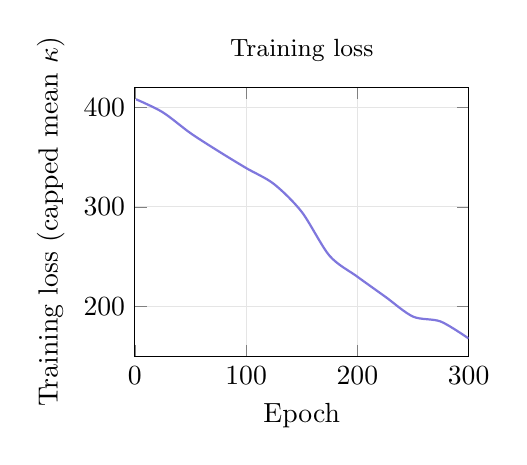
\begin{tikzpicture}
\begin{axis}[
  width=0.48\textwidth, height=5cm,
  xlabel={Epoch}, ylabel={Training loss (capped mean $\kappa$)},
  xmin=0, xmax=300, ymin=150, ymax=420,
  grid=major, grid style={gray!20},
  title={Training loss},
  title style={font=\small},
]
\addplot[cPurple, thick, smooth, no marks]
  coordinates {
    (1,408) (25,395) (50,374) (75,356) (100,339)
    (125,323) (150,295) (175,251) (200,230) (225,210)
    (250,190) (275,185) (300,168)
  };
\end{axis}
\end{tikzpicture}%
\hfill%
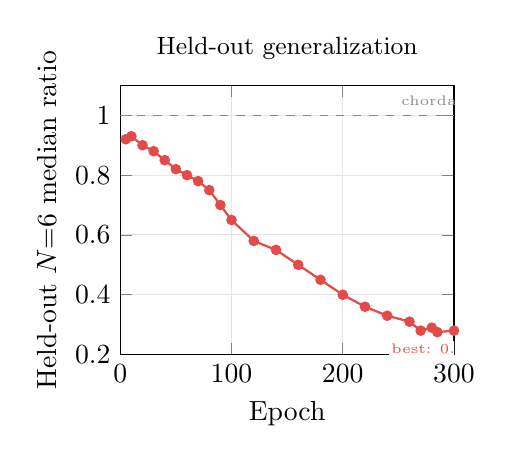
\begin{tikzpicture}
\begin{axis}[
  width=0.48\textwidth, height=5cm,
  xlabel={Epoch},
  ylabel={Held-out $N{=}6$ median ratio},
  xmin=0, xmax=300, ymin=0.2, ymax=1.1,
  grid=major, grid style={gray!20},
  title={Held-out generalization},
  title style={font=\small},
]
\addplot[cRed, thick, mark=*, mark size=1.5pt]
  coordinates {
    (5,0.92) (10,0.93) (20,0.90) (30,0.88) (40,0.85)
    (50,0.82) (60,0.80) (70,0.78) (80,0.75) (90,0.70)
    (100,0.65) (120,0.58) (140,0.55) (160,0.50)
    (180,0.45) (200,0.40) (220,0.36) (240,0.33)
    (260,0.31) (270,0.28) (280,0.29) (285,0.275) (300,0.28)
  };
\addplot[cGray, dashed, no marks, domain=0:300] {1.0};
\node[font=\tiny, text=cGray] at (axis cs:280,1.05) {chordal};
\node[font=\tiny, text=cRed, fill=white, inner sep=1pt]
  at (axis cs:285,0.22) {best: 0.275};
\end{axis}
\end{tikzpicture}
\caption{%
  Left: training loss decreases monotonically over 300 epochs. Right:
  held-out $N = 6$ median curvature ratio tracks training loss with no
  overfitting plateau, reaching 0.275 at epoch 285.%
}
\label{fig:trajectory}
\end{figure}


% ════════════════════════════════════════════════════════════════════════════
\section{Analysis}
\label{sec:analysis}


% ── 7.1 Encoder probing ──────────────────────────────────────────────────
\subsection{What Does the Encoder Learn?}

Linear probes (Ridge regression) on the encoder's intermediate
representations reveal that the model explicitly encodes geometric
quantities:

\begin{table}[h]
\centering
\caption{Linear-probe $R^2$ on encoder representations.}
\label{tab:probing}
\begin{tabular}{lc}
\toprule
\textbf{Target quantity} & $R^2$ \\
\midrule
Sequence position $i/N$ & 1.00 \\
Centripetal fraction $t_{\text{cp}}(i)$ & 0.99 \\
Chord fraction $t_{\text{chord}}(i)$ & 0.98 \\
Turning angle $\theta(i)$ & 0.82 \\
Local curvature $\kappa(i)$ & 0.76 \\
Non-local curvature $\kappa(i{+}2)$ & 0.71 \\
\bottomrule
\end{tabular}
\end{table}

All six geometric properties are recoverable above the $R^2 = 0.5$
threshold. The thesis's per-dof MLPs received these as hand-crafted input
features; the Transformer learns them from raw point coordinates through
attention.


% ── 7.2 Addressing §7.3 ─────────────────────────────────────────────────
\subsection{Addressing the §7.3 Limitation}

The prior work identified two parts to the fixed-input-size limitation:

\begin{enumerate}
  \item \textbf{Variable-length model} --- fully addressed.
        Padding masks in the encoder and DETR-style queries in the decoder
        handle any $N \leq N_{\max}$.
  \item \textbf{Batched variable-length energy layer} --- partially
        addressed.
        The N-grouped solver processes each length-group within a batch as
        a single batched call, but still loops over groups. A full
        jagged-tensor implementation remains future work.
\end{enumerate}


% ════════════════════════════════════════════════════════════════════════════
\section{Limitations and Future Work}
\label{sec:limitations}

\textbf{Output-head design.}
The cumsum-of-softplus normalization~\eqref{eq:output_head} pins the
$K$-th predicted knot to a value near $c_K / c_{K+1}$. While the slack
slot prevents exact pinning to 1.0, we observed that an earlier version
without the slack slot degenerated. A boundary rescaling
($\epsilon_b = 0.02$) is applied at evaluation. A proper fix
(autoregressive head or beta-distribution parameterization) is future work.

\textbf{2D only.}
All experiments use planar ($d = 2$) point sequences. The solver
(\texttt{curvature\_layer\_nd.py}) supports arbitrary dimension; extending
to 3D is straightforward in principle but untested.

\textbf{Random uniform data.}
Training and test data are random points in $[-0.5, 0.5]^2$. Evaluation
on real-world geometric data (CAD outlines, handwriting strokes, robot
trajectories) is needed to confirm practical utility.

\textbf{Single baseline.}
We compare against chordal parameterization only. The thesis additionally
compared centripetal, uniform, supervised, and line-search-optimal
baselines. Adding these comparisons would strengthen the empirical claims.

\textbf{Amortization gap.}
The model performs amortized optimization---one forward pass per sample.
It does not guarantee convergence to a local minimum. A hybrid approach
(Transformer initialization + gradient refinement) would close this gap
and likely improve results further.


% ════════════════════════════════════════════════════════════════════════════
\section{Conclusion}
\label{sec:conclusion}

We have shown that a single encoder--decoder Transformer, trained on
point sequences of length $N \in \{4, 5\}$ using a self-supervised
curvature objective, generalizes to held-out lengths $N = 6, 7, 8$
without retraining. On the held-out $N = 6$ test set, the model
achieves $75.7\% \pm 4.0\%$ win rate against the chordal heuristic
(3 seeds), with median curvature $\sim$70\% lower than the baseline.
On hard cases (chordal $\kappa > 1000$), the model produces curvature
2--6\% of chordal's, winning $\sim$90\% of the time.

These results demonstrate that a shared encoder can learn
length-invariant geometric structure rather than per-length patterns,
directly addressing the fixed-input-size limitation identified in
prior work. The contribution is architectural (one model for all
lengths), methodological (N-grouped batched energy layer), and
empirical (first evidence of length extrapolation in neural B-spline
parameterization).


% ════════════════════════════════════════════════════════════════════════════
% References
% ════════════════════════════════════════════════════════════════════════════
\begin{thebibliography}{9}

\bibitem{deBoor1978}
C.~de~Boor.
\newblock \emph{A Practical Guide to Splines}.
\newblock Springer-Verlag, 1978.

\bibitem{Lee1989}
E.~T.~Y.~Lee.
\newblock Choosing nodes in parametric curve interpolation.
\newblock \emph{Computer-Aided Design}, 21(6):363--370, 1989.

\bibitem{Chhetri2024}
V.~Chhetri.
\newblock \emph{Self-Supervised Learning for Optimal B-Spline
  Parameterization}.
\newblock Master's thesis, [University], 2024.

\bibitem{Carion2020}
N.~Carion, F.~Massa, G.~Synnaeve, N.~Usunier, A.~Kirillov, and
  S.~Zagoruyko.
\newblock End-to-end object detection with Transformers.
\newblock In \emph{ECCV}, 2020.

\bibitem{Vaswani2017}
A.~Vaswani, N.~Shazeer, N.~Parmar, J.~Uszkoreit, L.~Jones,
  A.~N.~Gomez, {\L}.~Kaiser, and I.~Polosukhin.
\newblock Attention is all you need.
\newblock In \emph{NeurIPS}, 2017.

\bibitem{Piegl1997}
L.~Piegl and W.~Tiller.
\newblock \emph{The NURBS Book}.
\newblock Springer, 2nd edition, 1997.

\bibitem{Laube2018}
P.~Laube, M.~O.~Franz, and G.~Umlauf.
\newblock Deep learning parametrization for B-spline curve approximation.
\newblock In \emph{3rd Intl.\ Conf.\ on Bio-engineering for Smart Technologies},
  2018.

\end{thebibliography}

\end{document}
